\documentclass[a4paper,12pt, italian]{article}
\usepackage{geometry}
\geometry{a4paper, top=3cm, bottom=3cm, left=2.5cm, right=2.5cm, heightrounded, bindingoffset=5mm}
\usepackage[italian]{babel}
\usepackage[version=3]{mhchem} 
\usepackage{siunitx} 
\usepackage{graphicx}
\usepackage{booktabs}
\usepackage{natbib} 
\usepackage{amsmath}
\usepackage{hyperref}
%\usepackage[labelformat=empty]{caption}
\setlength\parindent{15pt}
\usepackage{natbib}
\usepackage{amscd}
\usepackage{siunitx}
\usepackage{booktabs}
\usepackage{multicol}
\usepackage{tikz}
\usepackage{amsmath,amssymb}
\usepackage{amsthm}
\usepackage{tikz}
\usepackage{cancel}
\usepackage{float}
\usepackage{placeins} %aggiungi questo package e usa \FloatBarrier all'inizio e alla fine della sequenza di tabelle
\usepackage[labelsep=space]{caption} 
\renewcommand{\labelenumi}{\alph{enumi}.} 
\newcommand{\minitab}[2][l]{\begin{tabular}#1 #2\end{tabular}}
\newcommand{\angstrom}{\mbox{\normalfont\AA}}

\title{\textsc{Verifica della Legge di Ohm\\
Studio delle resistenze\\
Caratterizzazione corrente-tensione di un dispositivo non lineare}}
\date{}

\author{Laura \textsc{Trombetta}\\ Alessandro Maria \textsc{Turturiello}\\Federico \textsc{Venturoli}} 



\begin{document}

\maketitle 

\begin{center}
\begin{tabular}{l r}
Eseguita il giorno: &  5 maggio 2022 \\ 
Gruppo T2A-4: & Trombetta Laura\\
& Turturiello Alessandro Maria \\
& Venturoli Federico \\ 

\end{tabular}
\end{center}
\begin{abstract}
Lo scopo dell'esperienza è stato quello di studiare il funzionamento di un circuito, attraverso la Legge di Ohm, a seconda della posizione di una o più resistenze. E' stato anche caratterizzato l'andamento tensione-corrente di un dispositivo non lineare, nel nostro caso un diodo.
\end{abstract}
\tableofcontents
\maketitle
\newpage

\section{Introduzione e descrizione dell'apparato sperimentale}
Per condurre l'esperienza ci siamo serviti di una Breadboard dotata di due boccole e di una griglia di fori in cui inserire i refori. La griglia è caratterizzata dalla presenza di quattro colonne indicate con i simboli "+" e "-", ciascuna equipotenziale, e altre venti colonne equipotenziali riga per riga, indicate con delle lettere. Lo strumento ci ha permesso di realizzare i circuiti su cui abbiamo condotto le diverse misure. Le componenti di circuito di cui ci siamo serviti sono state le resistenze, di cui abbiamo ricavato i valori tramite un \textit{tool online}\footnote{ https://www.digikey.it/it/resources/conversion-calculators/conversion-calculator-resistor-color-code}, diodi di silicio e un partitore resistivo, composto da boccole e da interruttori in grado di modificare la resistenza dello strumento.
Abbiamo fatto uso di due multimetri, strumenti in grado di misurare diverse grandezze, nel nostro caso utilizzati per determinare la differenza di potenziale tra due punti del circuito e l'intensità di corrente.
Infine, abbiamo collegato un generatore che fornisse corrente ai circuiti, attraverso il controllo della sua differenza di potenziale.

\begin{figure}[h!]
    \centering
    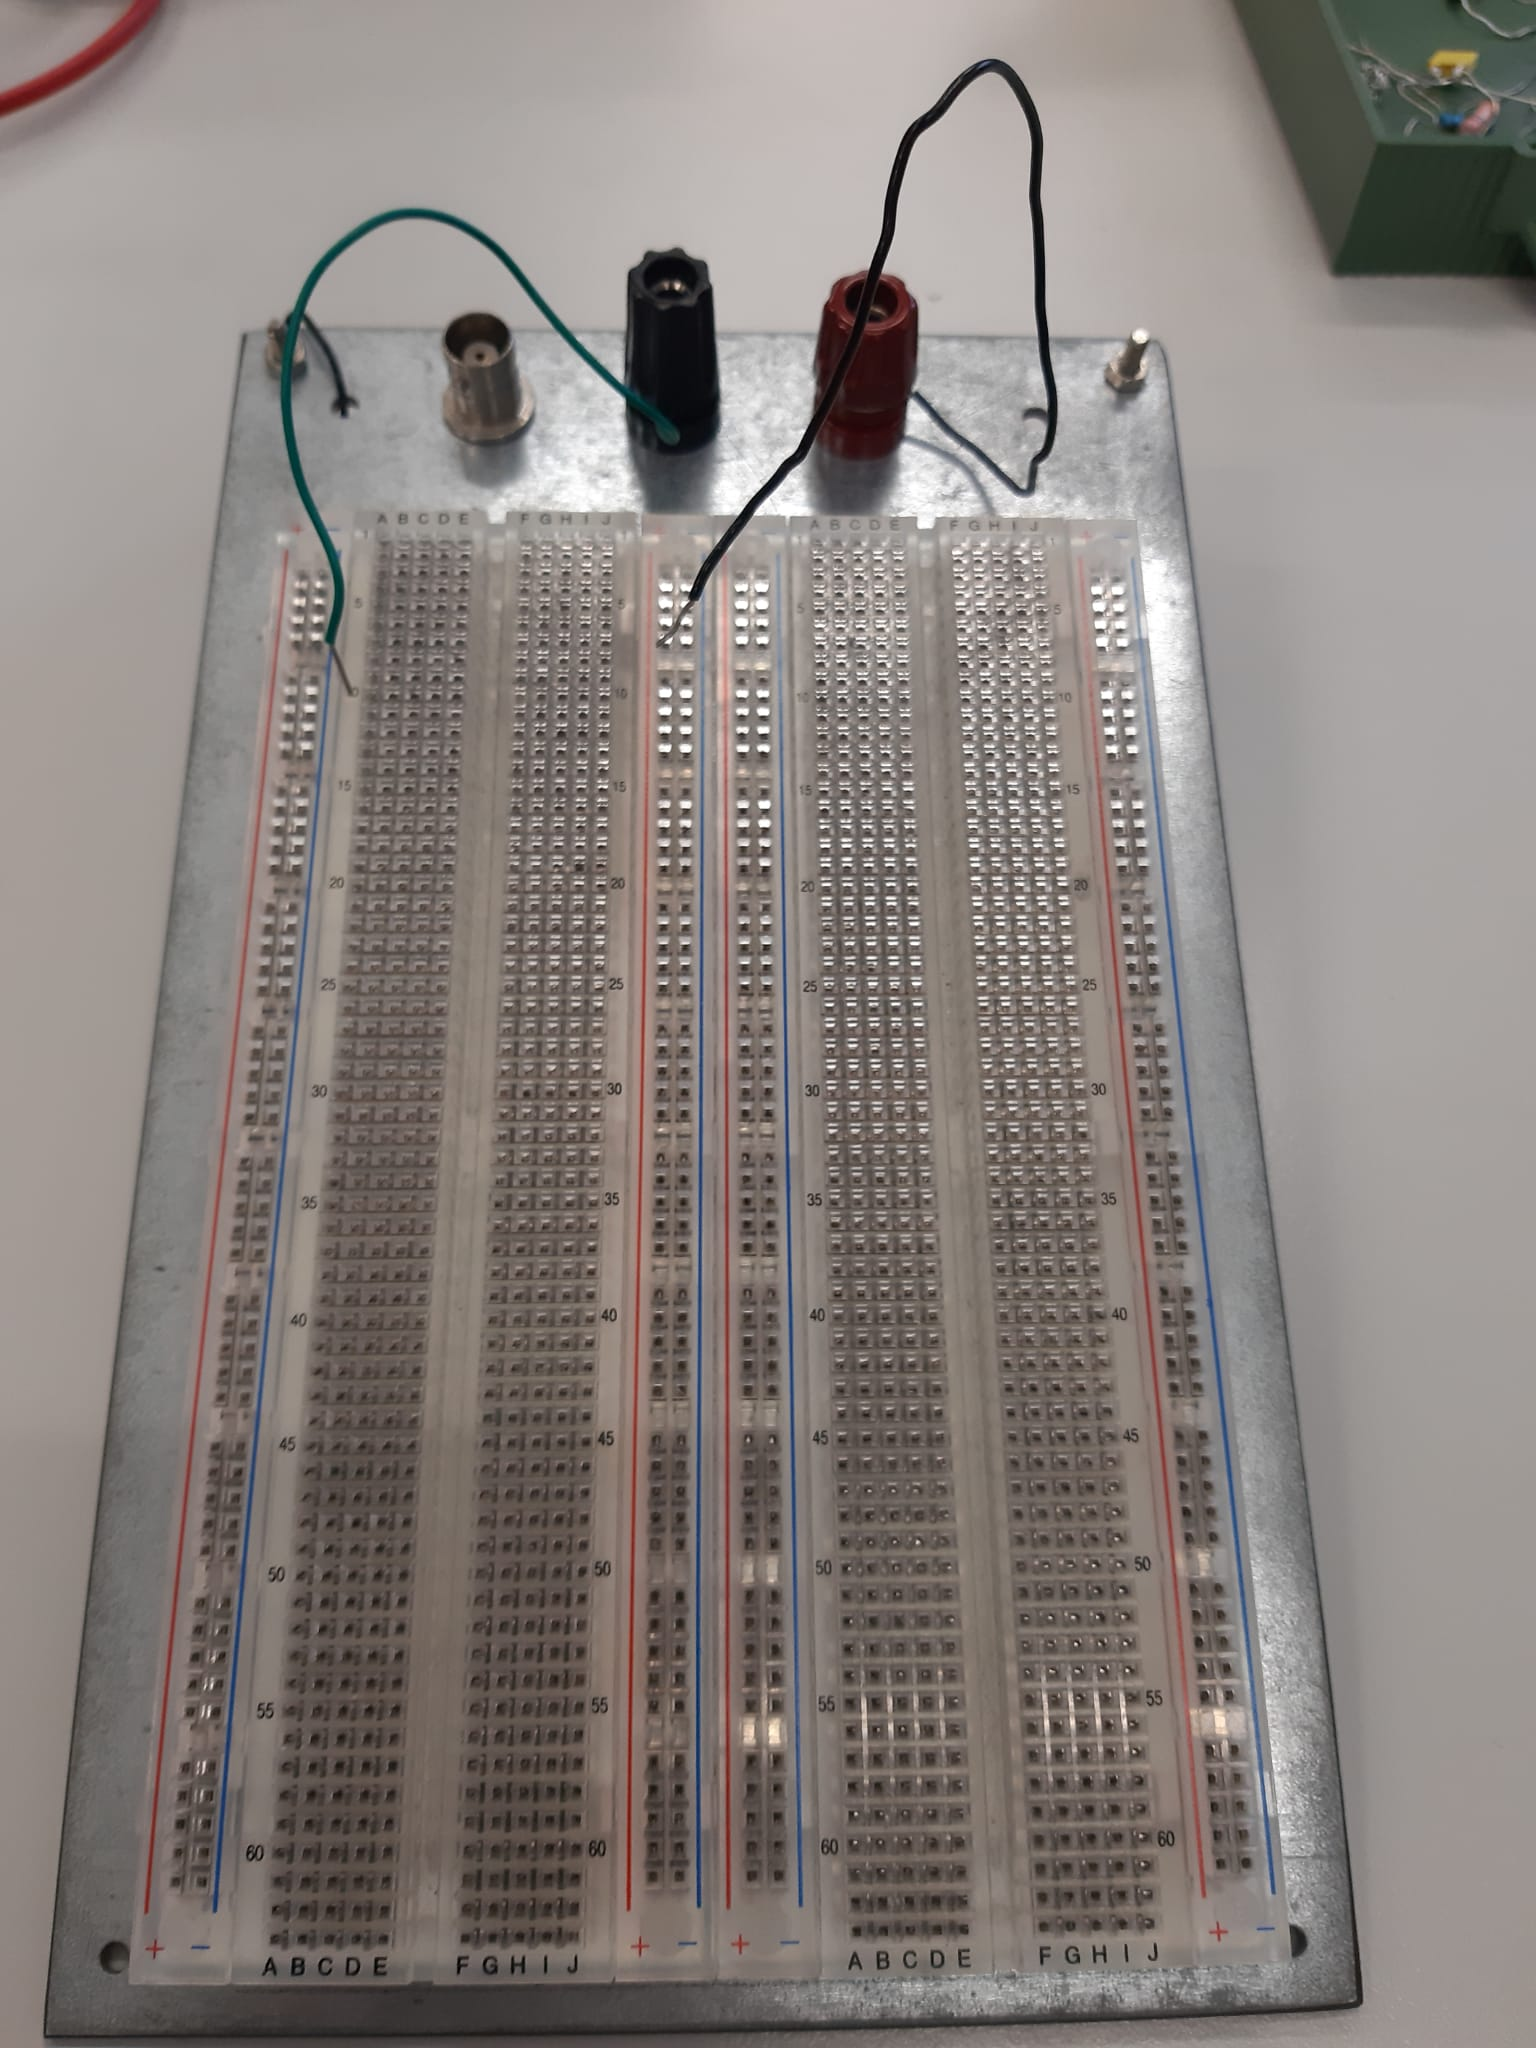
\includegraphics[scale=0.1]{Immagini/Circuitoooo.jpeg}
    \label{fig:my_label}
\end{figure}

La prima parte dell'esperienza si è concentrata sullo studio della strumentazione di laboratorio, studio finalizzato ad utilizzare configurazioni adeguate nelle parti successive. E' stato, infatti, necessario verificare che il multimetro usato come Voltmetro fosse ben progettato, cioè che avesse la caratteristica di possedere una resistenza in parallelo grande. Analogamente, è stato necessario verificare che il multimetro usato come Amperometro avesse la caratteristica di possedere una resistenza in serie piccola.
Successiavmente ci siamo concenrati sullo studio delle resistenze e della Legge di Ohm:

\begin{equation}
\frac{1}{R_{\parallel}}=\sum_{i=1}^{N}\frac{1}{R_{i}} \hspace{73 pt} R_{\perp}=\sum_{i=1}^{N}R_{i}
\end{equation}

\begin{equation}
V=R_{tot}I
\end{equation}

Infine, abbiamo studiato la Legge di Shockley, che descrive l'andamento di corrente per i diodi:

\begin{equation}
I=I_{0}(e^{qv/gK_b T}-1)
\end{equation}

indicando con \textit{q} la carica degli elettroni, con $K_b$ la costante di Boltzmann, con \textit{g} la costante che dipende dal tipo di diodo e con T la temperatura del diodo in Kelvin, corrispondente a quella dell'ambiente. Il termine di proporzionalità $I_0$ è detto \textit{intensità di corrente di saturazione}, il valore che ci aspettiamo di ottenere è molto piccolo in quanto si tratta di una corrente generata dai portatori di carica interni al diodo in diffusione dalla regione neutra alla regione di carica spaziale\footnote{Si tratta di una regione isolante all'interno di un semiconduttore drogato.}.
\section{Misura della caratteristica corrente-tensione di un resistore}
\subsection{Misura resistenza Voltmetro e Amperometro}
Per verificare che i lettori di grandezza di cui disponevamo fossero ben progettati, abbiamo proceduto analizzando due configurazoni differenti di circuiti.

Nella prima configurazione abbiamo disposto gli elementi circuitali come in figura:

\begin{figure}[h!]
    \centering
    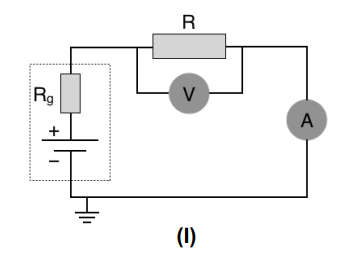
\includegraphics[scale=1]{Immagini/Conf1.PNG}
    \label{fig:my_label}
\end{figure}

Un lettore di tensione ideale dispone di una resistenza infinita; poichè nel caso reale non è possibile riporodurre questo fenomeno, si scelgono per i circuiti resistenze di ordini di grandezza molto minori di quelle dello strumento.
Abbiamo scelto la resistenza R, disposta in parallelo con quella del Voltmetro $R_{V}$, con un valore di $R=22M\Omega$. Questa scelta è stata motivata dal fatto che, per poter in seguito utilizzare resistenze con valori adatti, è stato necessario misurare quella del Voltmetro, confrontandola con un resistore che avesse un ordine di grandezza simile.
Riportiamo di seguito i dati raccolti, utilizzati per condurre un'interpolazione.

\begin{table}[H]
    \centering
    \begin{tabular}{cc}
    \toprule
    \Delta V (V)  & I (\mu A) \\
    \midrule
    0,507	&0,59\\
    1,012	&1,20\\
    1,527	&1,83\\
    2,032	&2,43\\
    2,544	&3,04\\
    3,051	&3,65\\
    3,56	&4,27\\
    \bottomrule
    \end{tabular}
    \label{tab:my_label}
\end{table}
 
\begin{figure}[H]
    \centering
    %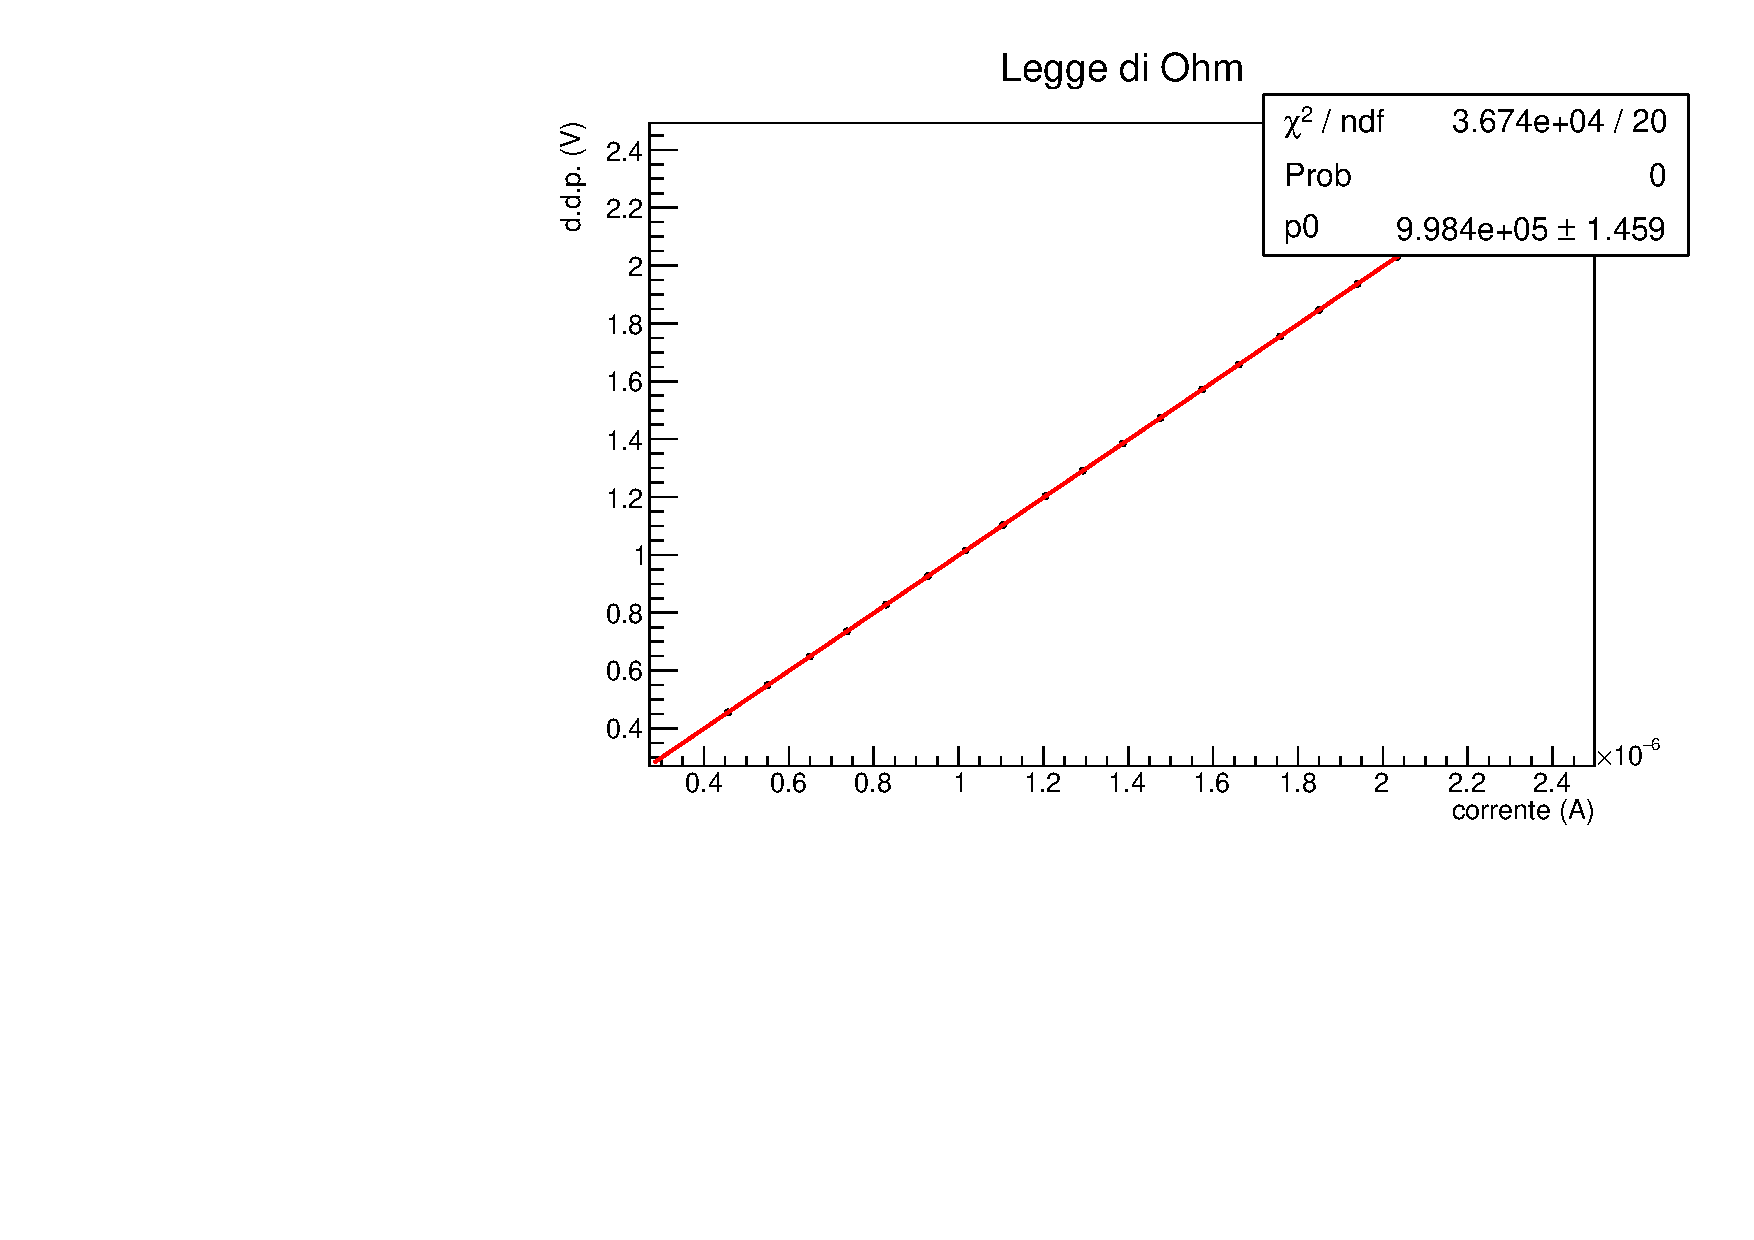
\includegraphics[scale=.5]{Immagini/Ohm configurazione 1.pdf}
    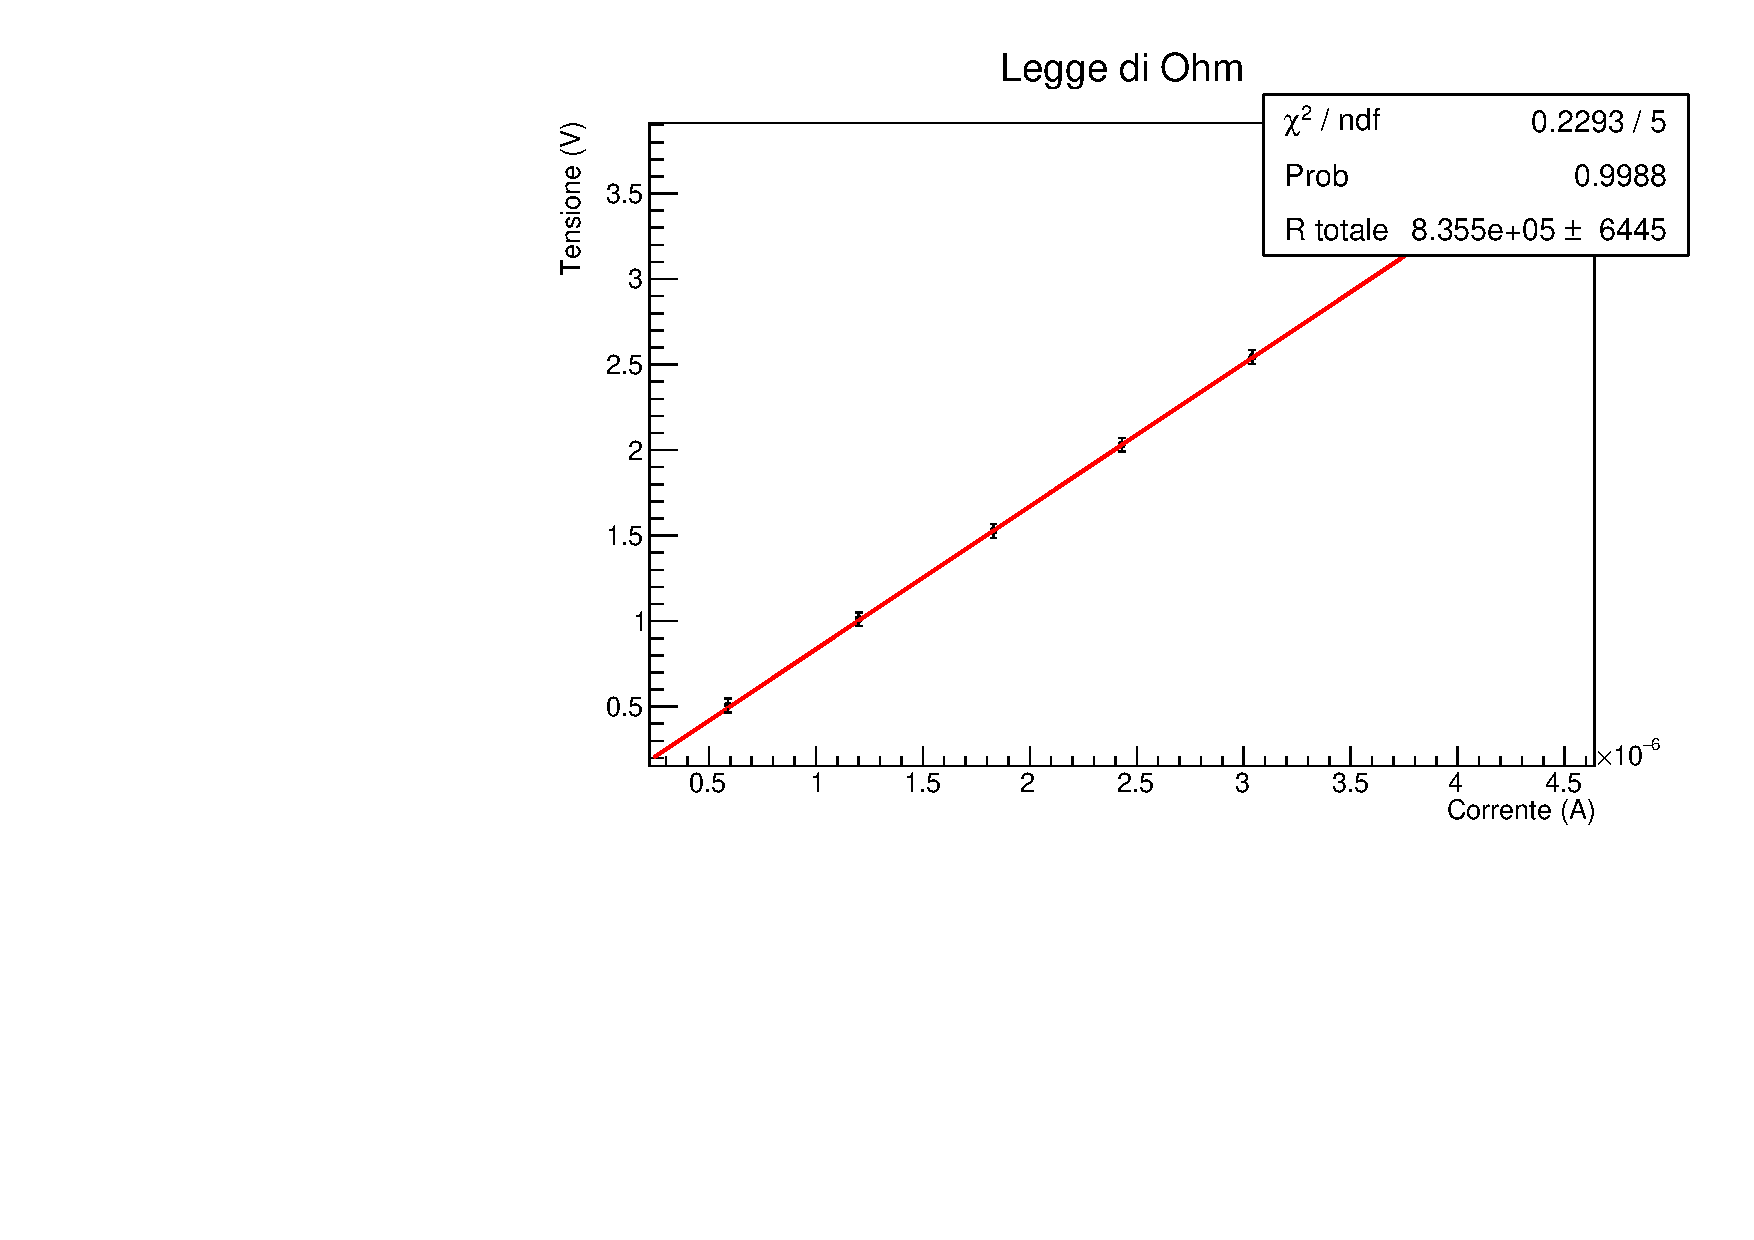
\includegraphics[scale=.5]{Immagini/fit1.pdf}
    \label{fig:my_label}
    \caption{Grafico configurazione Voltmetro}
\end{figure}

La resistenza del Voltmetro risulta essere di $1,05M\Omega$, essa dovrebbe, però, essere dell'ordine di grandezza di 10 $M\Omega$; discuteremo i motivi di questa incongruenza nelle conclusioni, ma crediamo possa essere attribuibile alla resistenza nota scelta.

Per il calcolo dell'errore abbiamo operato come segue:

$$
\sigma_{R_v}^2=\left[\sigma_{R_{equiv}}\left(\dfrac{\partial R_v}{\partial R_{equiv}}\right)\right]^2=\sigma^2_{R_{equiv}}\left(\dfrac{R_v^2}{(R_n -R_{tot}^2)}\right)^2=2,322 \Omega
\qquad \text{}
$$


Nella seconda configurazione abbiamo disposto gli elementi circuitali come in figura:

\begin{figure}[H]
    \centering
    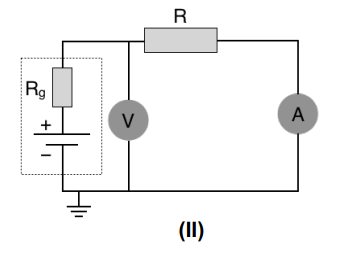
\includegraphics[scale=1]{Immagini/Conf2.PNG}
    \label{fig:my_label}
\end{figure}

Abbiamo scelto la resistenza R, disposta in serie con quella del Amperometro $R_{A}$, con un valore di $R=10\Omega$ per un motivo simile al precedente. A differenza del Voltmetro, l'Amperometro ideale ha una resistenza nulla, quindi, nella realtà, si scelgono resistori di ordini di grandezza molto maggiori dello strumento.
Anche in questo caso abbiamo deciso di condurre un'interpolazione per ricavare la resistenza equivalanente e, successivamente, quella dello strumento.

\begin{table}[H]
    \centering
    \begin{tabular}{cc}
    \toprule
    \Delta V (V)  & I (mA) \\
    \midrule
    1,016	&88,56\\
    1,515	&132,06\\
    2,026	&176,42\\
    2,533	&220,37\\
    3,044	&264,4\\
    3,549	&307,59\\
    4,061	&351,3\\
    \bottomrule
    \end{tabular}
    \label{tab:my_label}
\end{table}

\begin{figure}
    \centering
    %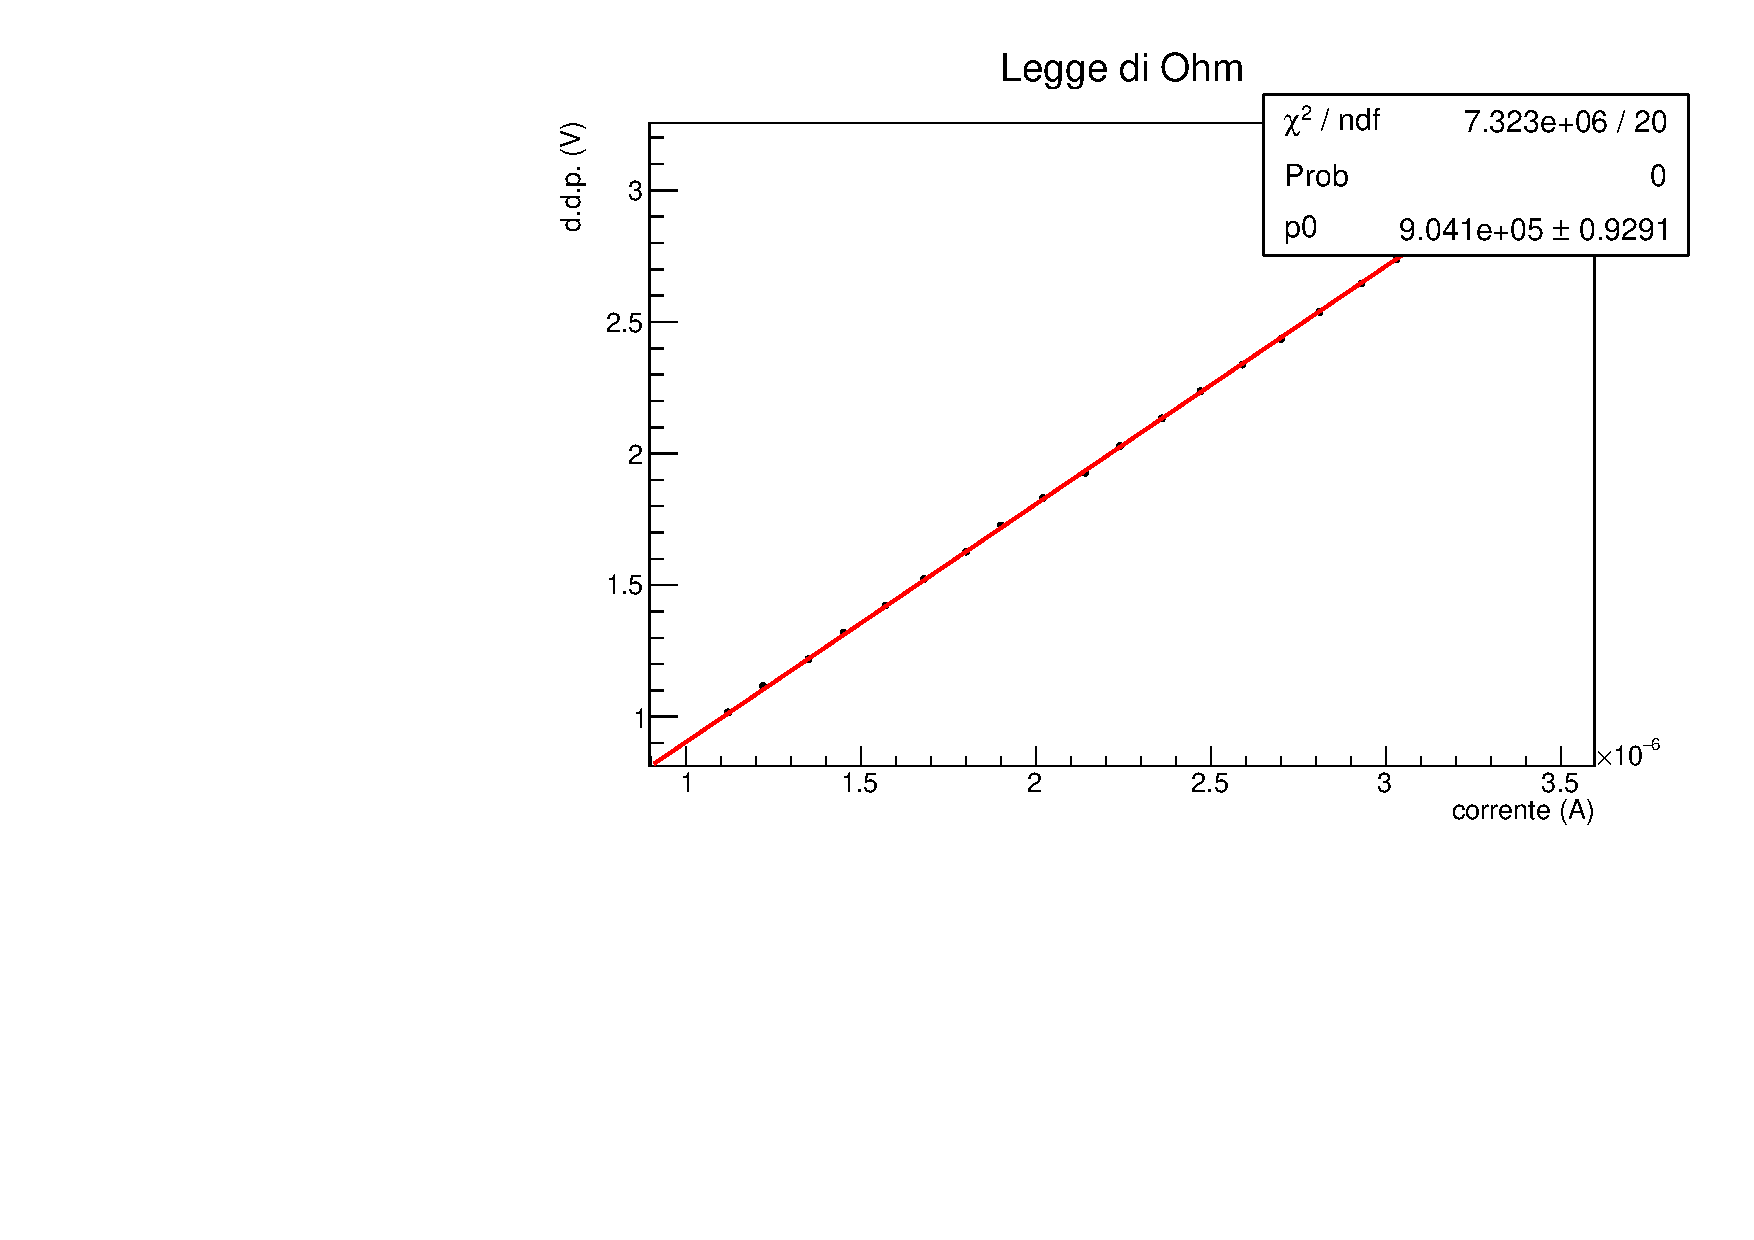
\includegraphics[scale=.5]{Immagini/Ohm configurazione 2.pdf}
    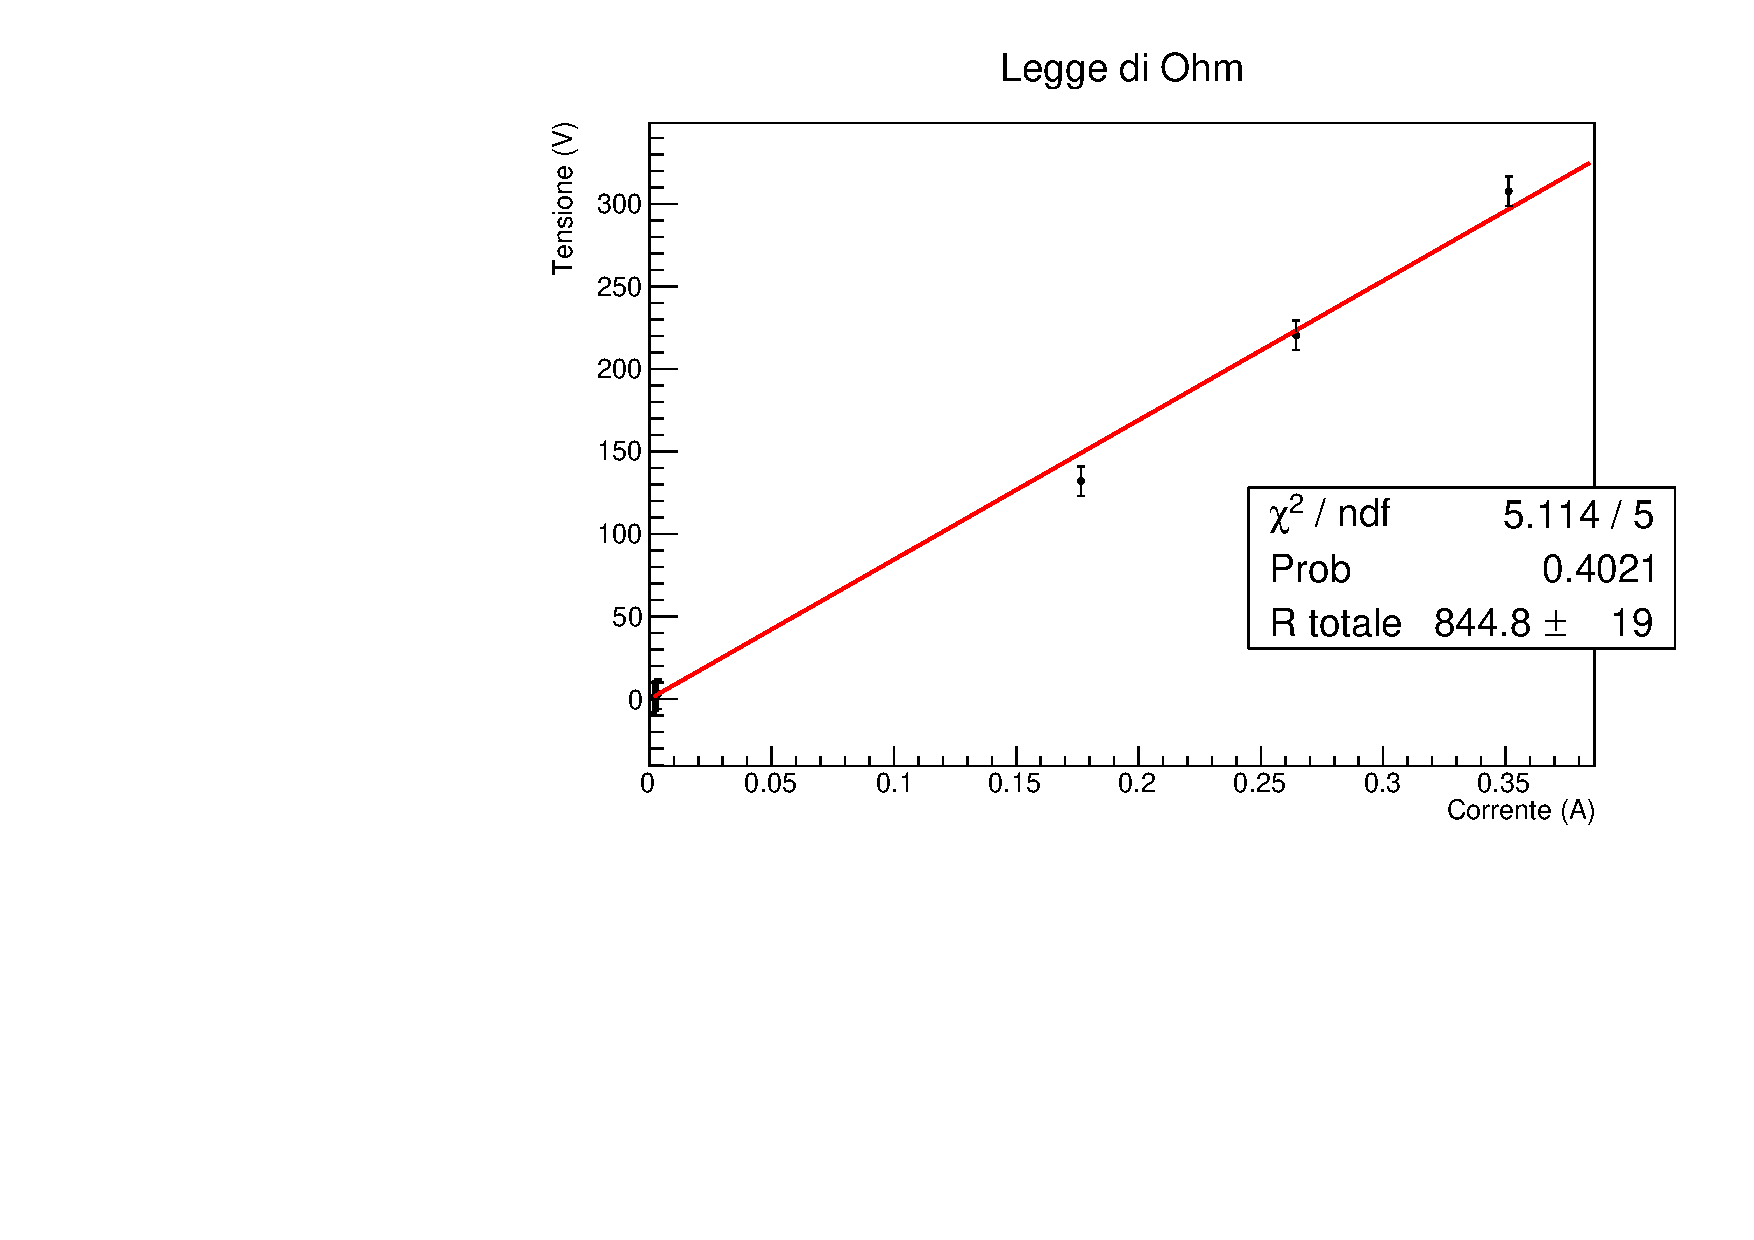
\includegraphics[scale=.5]{Immagini/fit2.pdf}
    \label{fig:my_label}
    \caption{Grafico configurazione Amperometro}
\end{figure}

Questo risultato risulta congruente con quello che ci aspettavamo.

\subsection{Verifica della legge di Ohm}
Successivamente, configurando correttamente entrambi i circuiti, abbiamo verificato la Legge di Ohm. Variando la misura della tensione di alimentazione del circuito, abbiamo misurato la differenza di potenziale ai capi del resistore e la corrente che lo attraversava.

\begin{table}[H]
\parbox{.45\linewidth}{
    \centering
    \begin{tabular}{cc|cc}
    \toprule
    \Delta V (V)  & I (mA) & \Delta V (V)  & I (mA) \\
    \midrule
    0,456	&0,45693 & 1,385	&1,3869\\
    0,55	&0,5497 & 1,474	&1,4761\\
    0,649	&0,6498 & 1,572	&1,5741\\
    0,736	&0,7372& 1,658	&1,6604\\
    0,828	&0,8293& 1,755	&1,7584\\
    0,927	&0,928& 1,847	&1,85\\
    1,015	&1,0166& 1,937	&1,9403\\
    1,103	&1,1048& 2,03	&2,0335\\
    1,203	&1,2048& 2,124	&2,128\\
    1,291	&1,293& 2,216	&2,2196\\
    2,308	&2,3126&&\\
    \bottomrule
    \end{tabular}
    \caption{Dati configurazione 1, R=1k\Omega}
    \label{tab:my_label}
}
\quad
\parbox{.45\linewidth}{
    \centering
    \begin{tabular}{cc|cc}
    \toprule
    \Delta V (V)  & I (\mu A) & \Delta V (V)  & I (\mu A) \\
    \midrule
    1,017	&1,12& 2,029	&2,24\\
    1,117	&1,22&2,134	&2,36\\
    1,219	&1,35& 2,237	&2,47\\
    1,319	&1,45&2,338	&2,59\\
    1,423	&1,57&2,436	&2,7\\
    1,524	&1,68&2,538	&2,81\\
    1,627	&1,8&2,646	&2,93\\
    1,727	&1,9&2,738	&3,03\\
    1,831	&2,02&2,85	&3,16\\
    1,927	&2,14&2,948	&3,27\\
    3,053	&3,37 &&\\
    \bottomrule
    \end{tabular}
    \caption{Dati configurazione 2, R=0,91M\Omega}
    \label{tab:my_label}
    }
\end{table}

\begin{figure}[H]
    \centering
    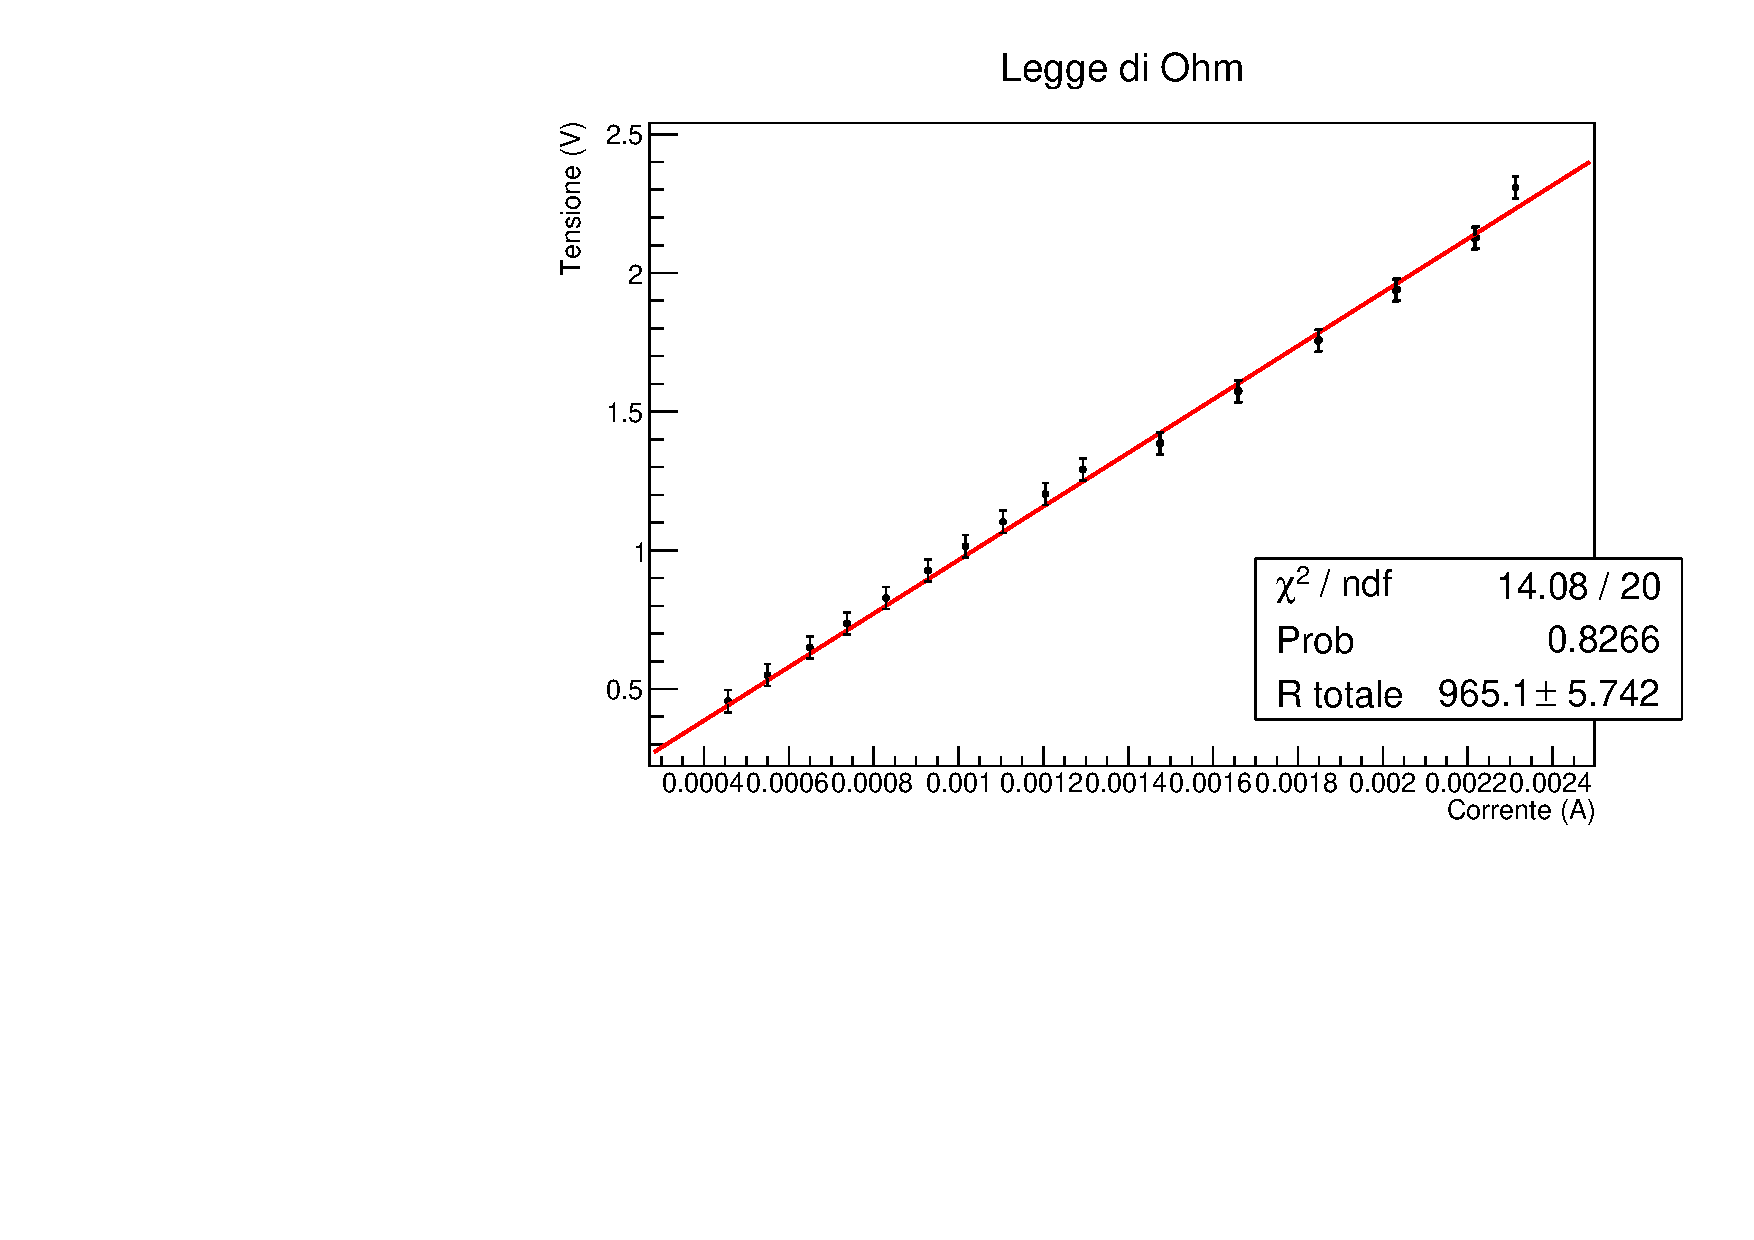
\includegraphics[scale=.45]{Immagini/fit3.pdf}
    \quad
    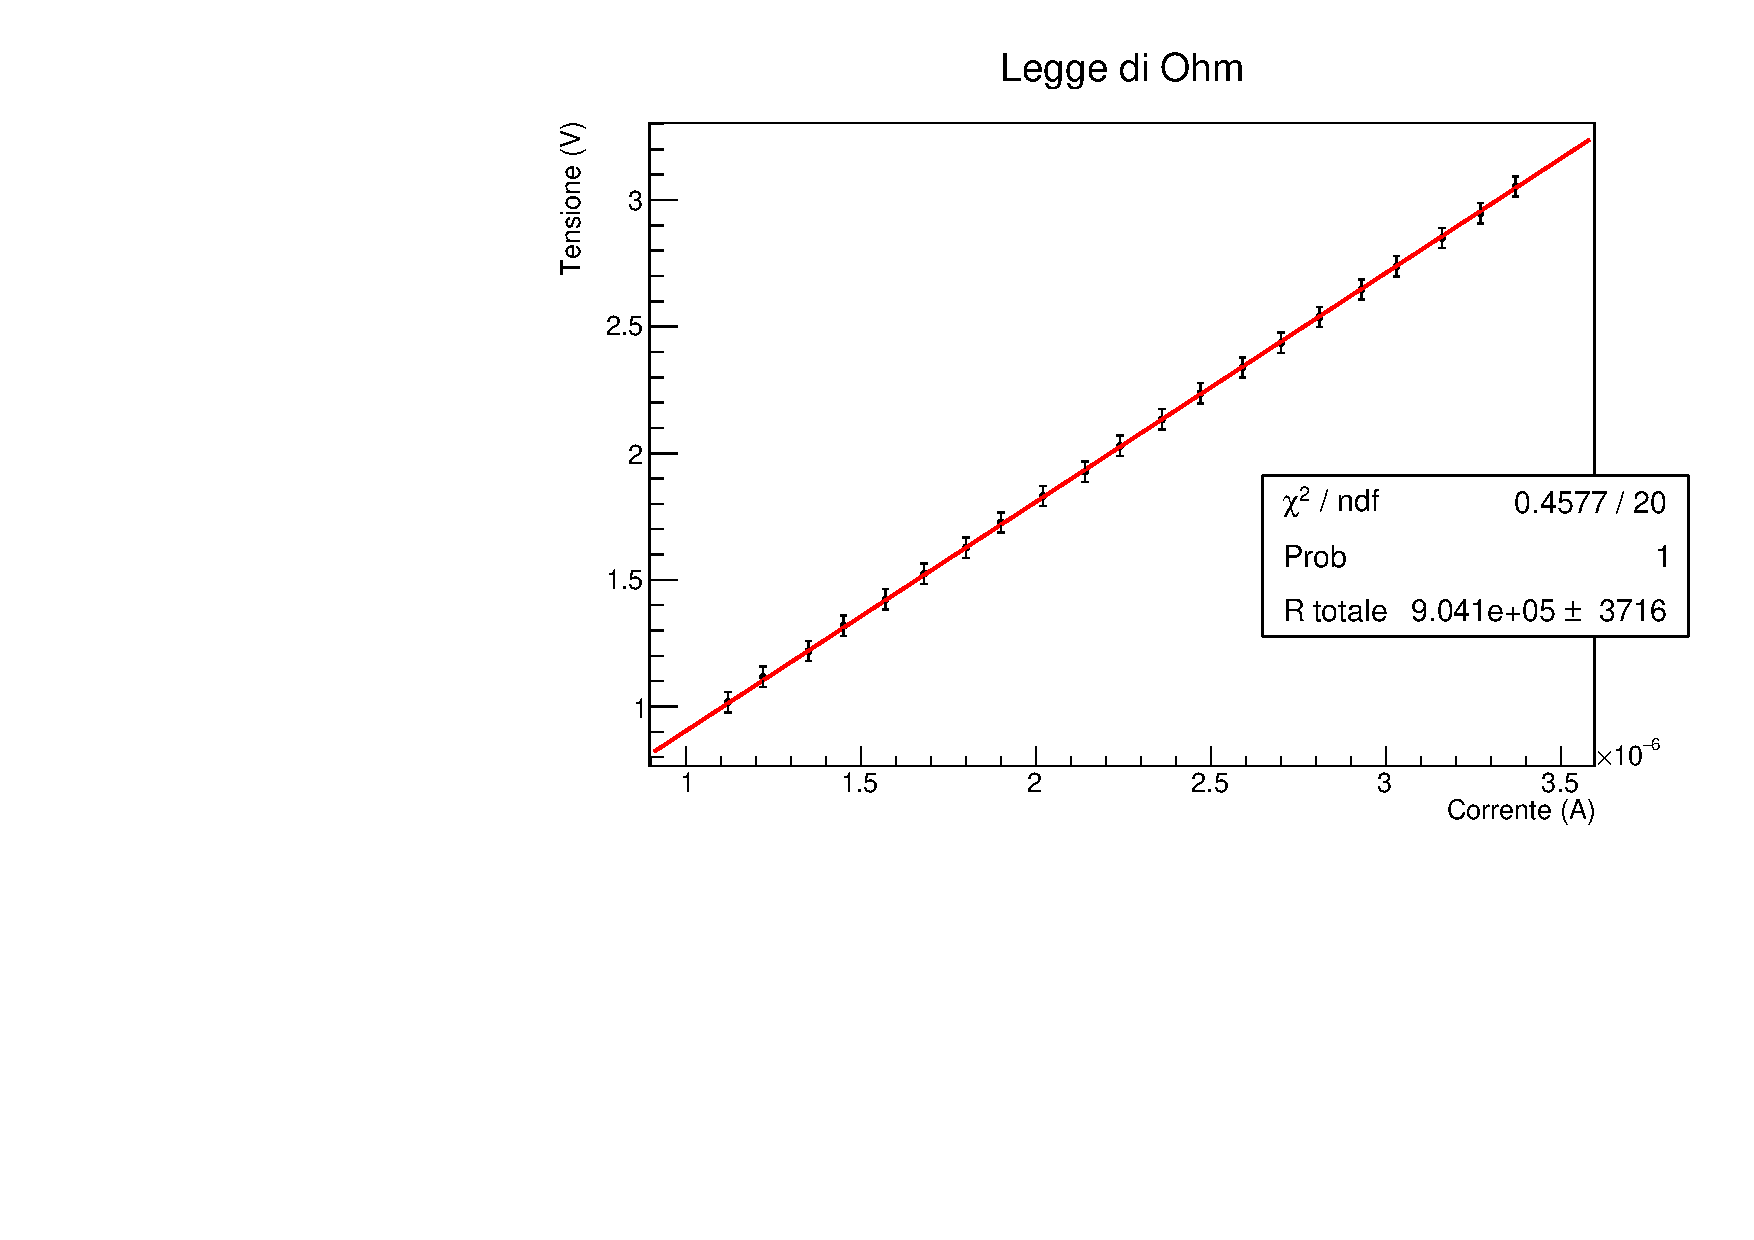
\includegraphics[scale=.45]{Immagini/fit4.pdf}
    \caption{Configurazione 1 in alto e configurazione 2 in basso}
\end{figure}


\subsection{Misura di resistenze composite}
Infine abbiamo disposto, prima in parallelo e poi in serie, due resistori (scelti con lo stesso ordine di grandezza della resistenza) e abbiamo verificato con essi la legge di Ohm. In questo caso abbiamo utilizzato solamente la configurazione 2, in quanto la misura che in precedenza avevamo ottenuto per $R_{V}$ poteva non essere corretta.

\begin{table}[H]
\parbox{.45\linewidth}{
    \centering
    \begin{tabular}{cc}
    \toprule
    $\Delta$ V (V)  & I (mA) \\
    \midrule
    0,503	&44,12\\
1,016	&89,15\\
1,519	&133,25\\
2,029	&177,94\\
2,538	&221,84\\
3,044	&265,8\\
3,551	&109,5\\
4,055	&352,8\\
    \bottomrule
    \end{tabular}
    \caption{Resistenze in parallelo; R_{tot}=5$\Omega$}
    \label{tab:my_label}
    }
    \quad
    \parbox{.45\linewidth}{
    \centering
    \begin{tabular}{cc}
    \toprule
    $\Delta$ V (V)  & I (mA) \\
    \midrule
    0,507	&23,916\\
1,016	&47,931\\
1,524	&71,92\\
2,029	&95,73\\
2,539	&119,76\\
3,048	&114,7\\
3,551	&167,36\\
4,065	&191,45\\
    \bottomrule
    \end{tabular}
    \caption{Resistenze in serie; R_{tot}=20$\Omega$}
    \label{tab:my_label}
    }
\end{table}
\noindent
I fit e i relativi risultati sono riportati nella Figura \ref{fit 56}.
\begin{figure}[h!]
    \centering
    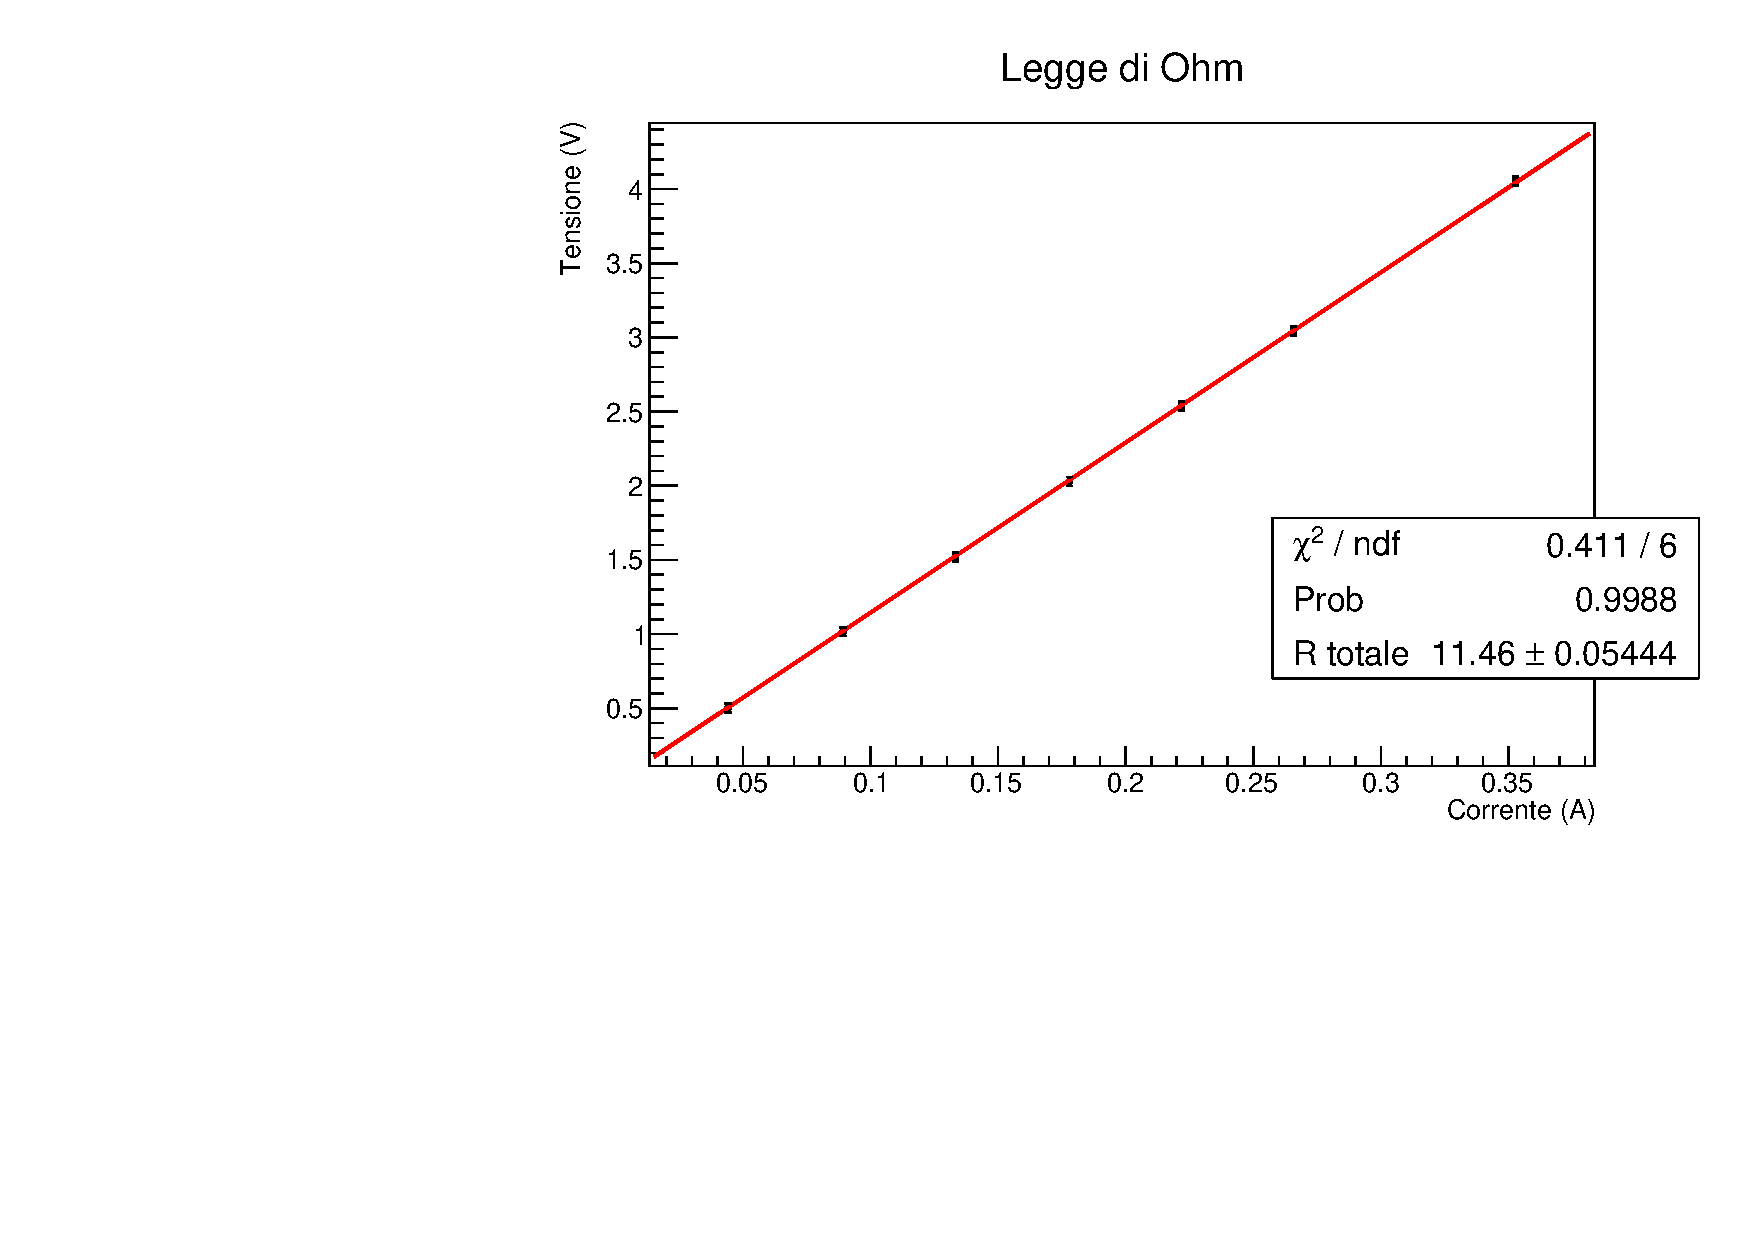
\includegraphics[scale=.4]{Immagini/fit5.pdf}
    \\
    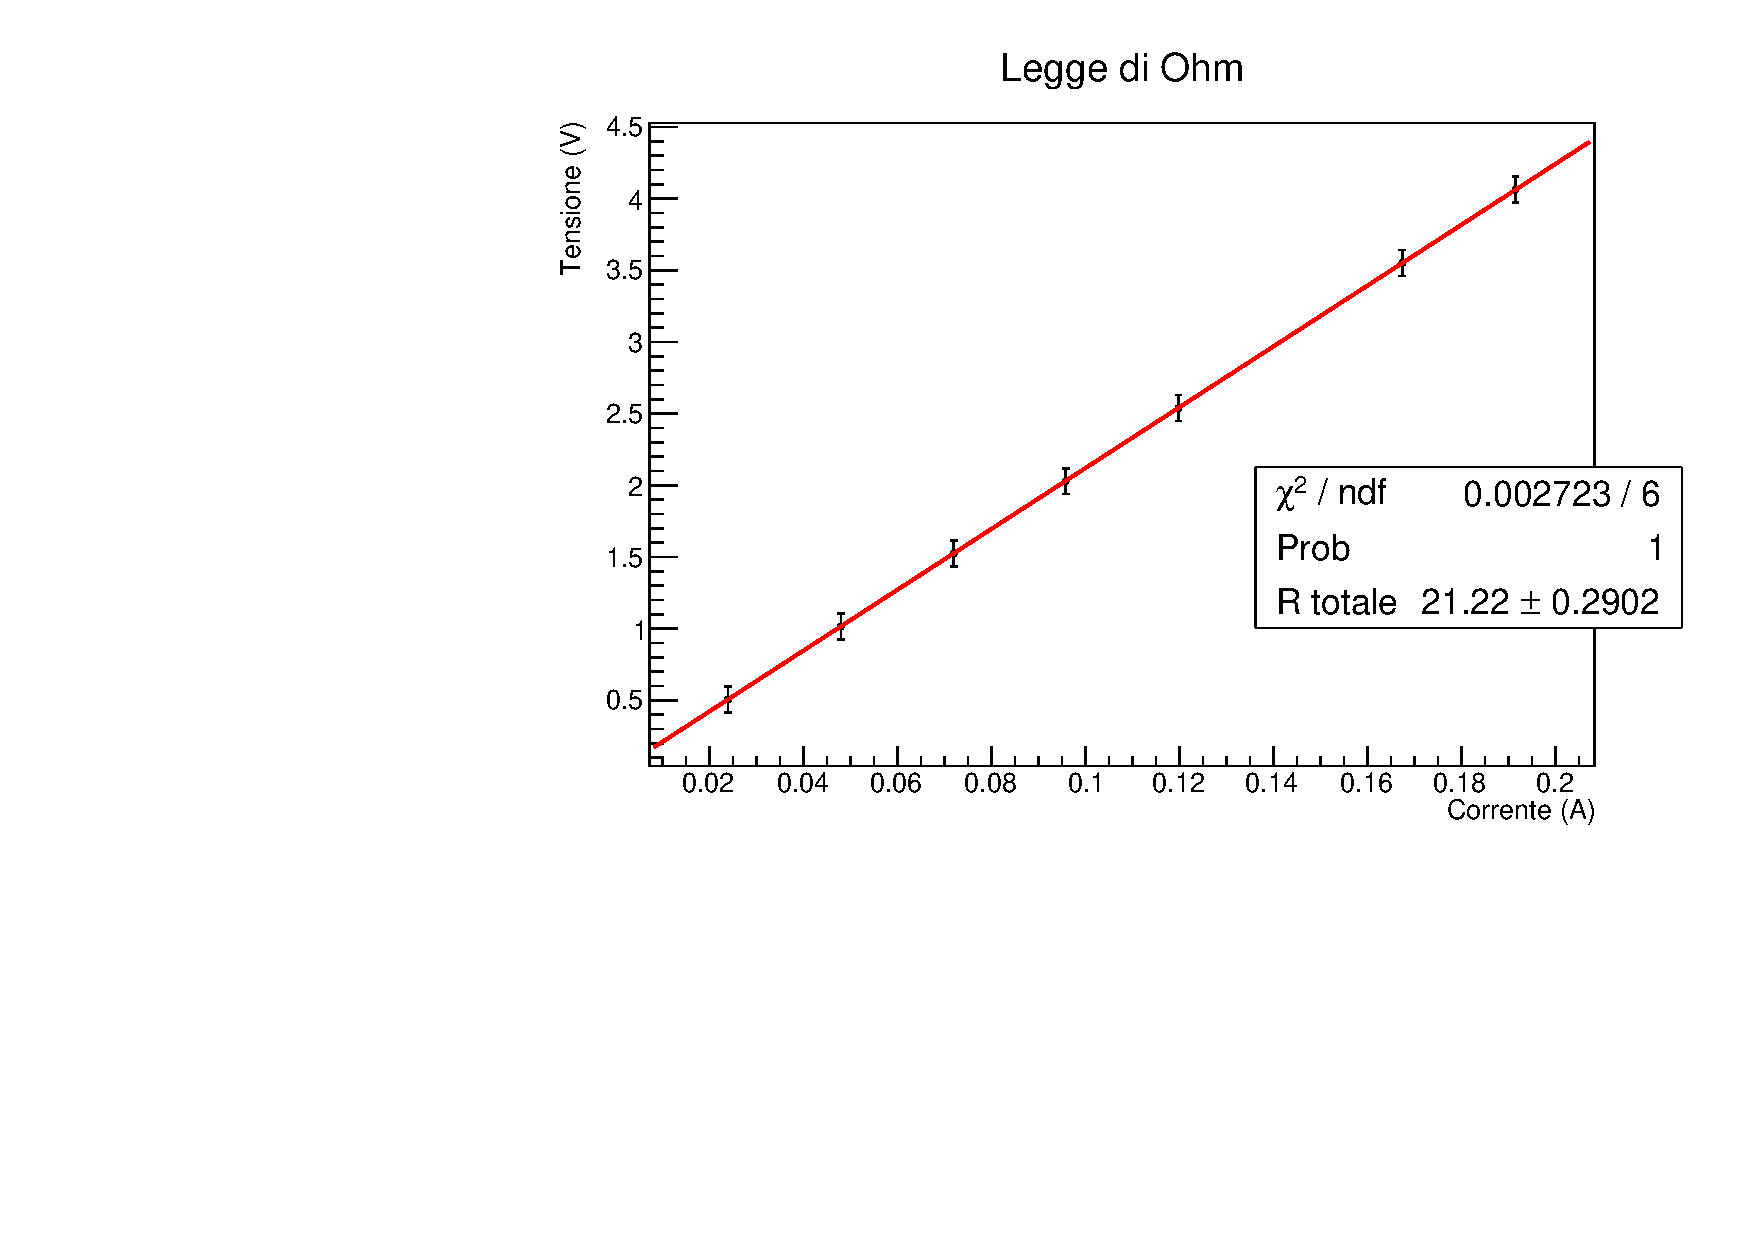
\includegraphics[scale=.4]{Immagini/fit6.pdf}
    \caption{}
    \label{fit 56}
\end{figure}
\section{Partitore resistivo}
In questa parte di esperienza abbiamo studiato la seguente configurazione:

\begin{figure}[H]
    \centering
    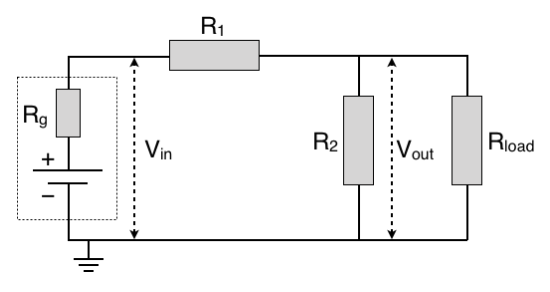
\includegraphics[scale=1]{Immagini/PartResist.PNG}
    \label{fig:my_label}
\end{figure}

nella quale con $R_{load}$ indichiamo il partitore resistivo, componente di circuito di cui è possibile scegliere la resistenza attraverso interruttori.
Abbiamo studiato la configurazione sotto la condizione in cui $V_{out}$ = 0.5$V_{in}$.
Attraverso considerazioni sulle resistenze equivalenti e sulla confrontabilità tra la resistenza del partitore e quelle note, siamo arrivati alla conclusione per la quale, al fine di avere una configurazione con la condizione sopra citata, era necessario che $R_{1}$ ed $R_{2}$ fossero uguali e che $R_{load}$ fosse mandata a infinito. Nella pratica, questa procedura è stata compiuta aumentando sempre più la resistenza del partitore.

\begin{equation}
R_{eq} = \frac{R_{2}R_{load}}{R_{2}+R_{load}} \hspace{73 pt} R_{tot} = R_{1}+\frac{R_{2}R_{load}}{R_{2}+R_{load}}
\end{equation}
\begin{equation}
\label{eq: 5}
V_{in} = R_{tot}I \hspace{73 pt} V_{out} = R_{eq}I = V_{in}\frac{R_{eq}}{R_{1}+R_{eq}}  
\end{equation}
\noindent
Dalla equazione \ref{eq: 5} è evidente che, nel caso in cui  $R_{load}\to \infty$ e $V_{out}$ = 0.5$V_{in}$, si ottiene \begin{equation}
\frac{1}{2} = \frac{R_{2}}{R_{1}+R_{2}} \hspace{20 pt} \text{per cui} \hspace{20 pt} R_{1} = R_{2}
\end{equation}

Abbiamo confermato queste osservazioni sperimentalmente (utilizzando come resistenze $R_{1} = R_{2} = 150k\Omega)$, come risulta visibile dal grafico:

\begin{figure}[H]
    \centering
    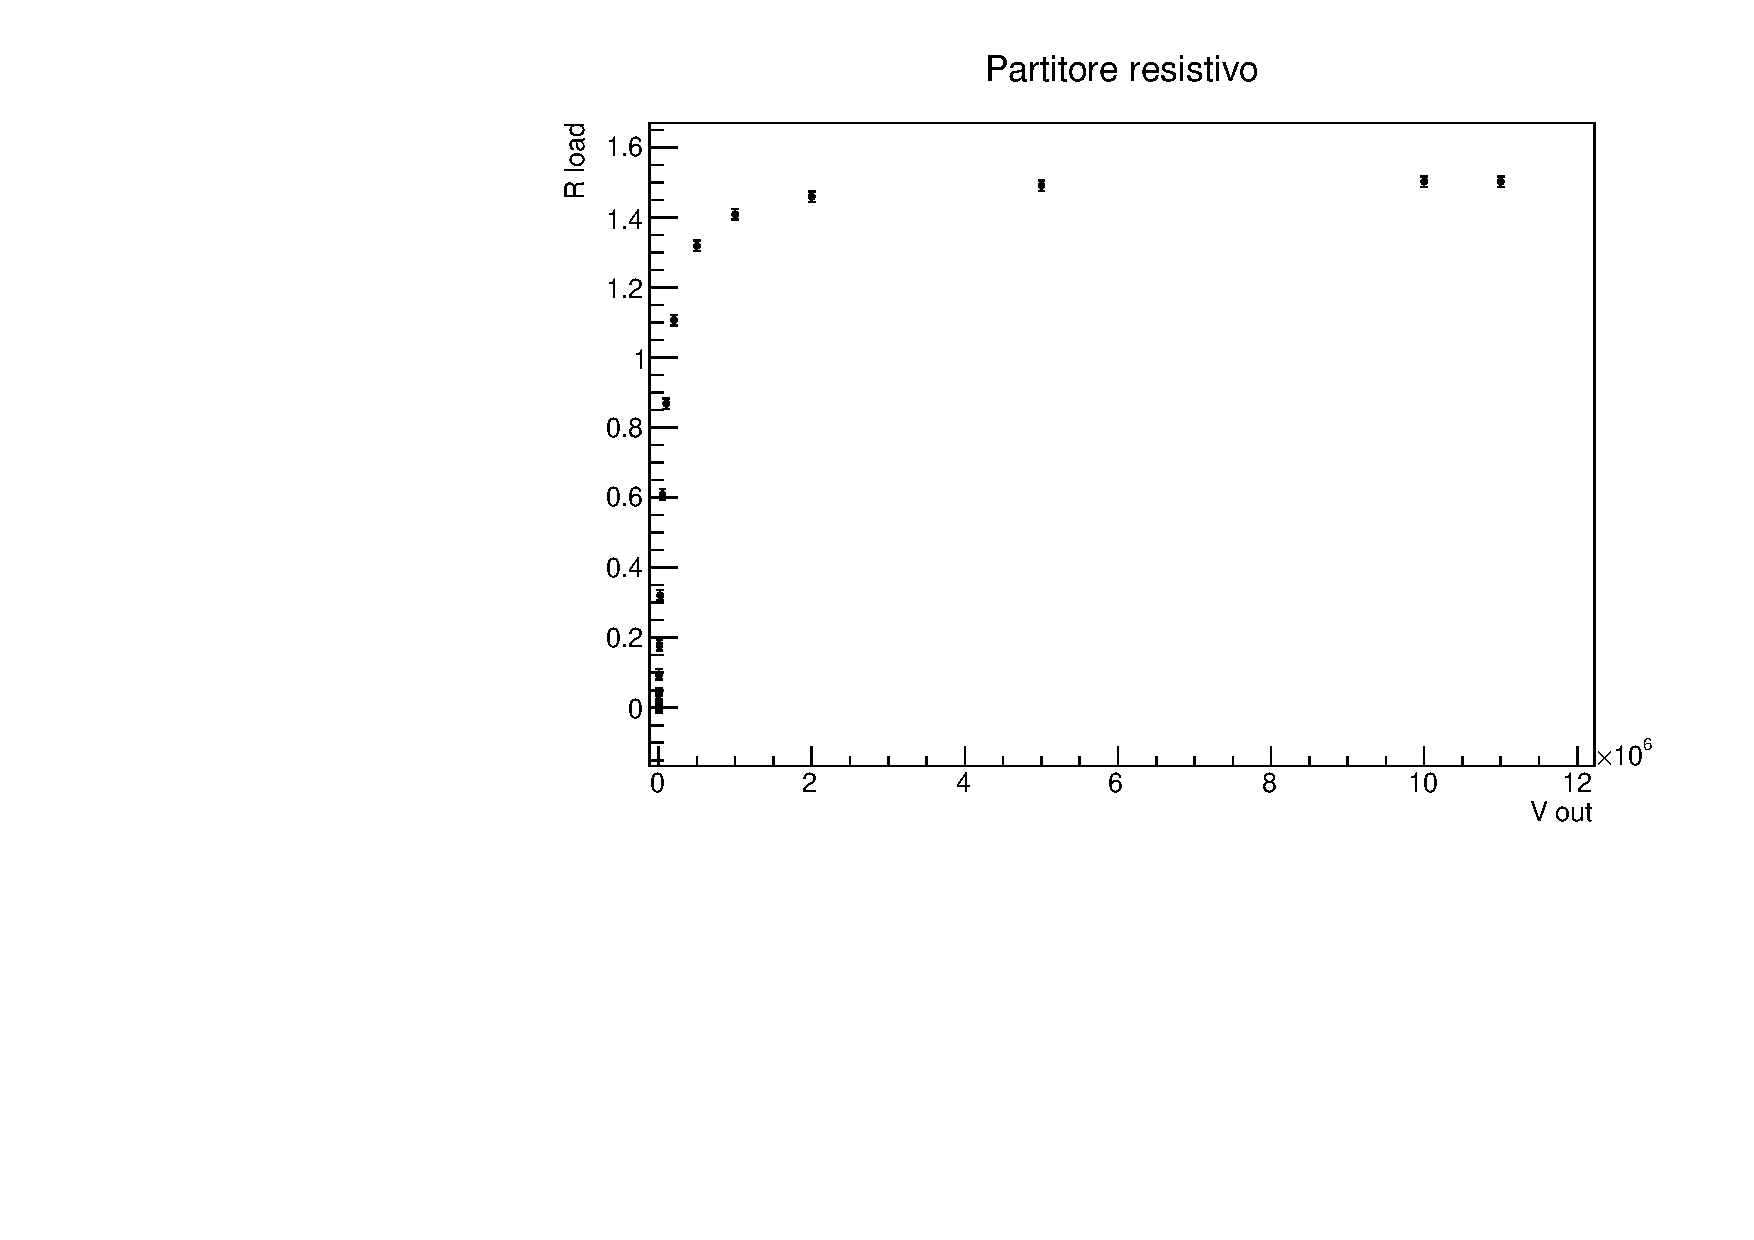
\includegraphics[scale=.6]{partitore resistivo.pdf}
    \caption{}
    \label{fig: partitore resistivo}
\end{figure}
\section{Misura della caratteristica corrente-tensione di un diodo}
In questa sezione abbiamo sostituito la resistenza nel circuito utilizzato in precedenza con un diodo. Esso è un elemento circuitale non lineare la cui funzione è quella di permettere alla corrente elettrica di fluire in un verso e di bloccarla quasi totalmente nell'altro.
Abbiamo proceduto variando la tensione di alimentazione del circuito, misurando la differenza di potenziale ai capi del diodo e la corrente che lo attraversava.
Nonostante la Legge di Shockley descriva l'andamento della corrente con una relazione esponenziale, nella realtà si usa definire una tensione di soglia, $V_{soglia}$, oltre la quale il diodo è considerato in conduzione.
In primis abbiamo verificato la legge sopra citata attraverso un fit esponenziale, in cui l'unico parametro era $I_{0}$, in quanto gli altri erano costanti o termini noti.
Di seguito è riportato il fit esponenziale

\begin{figure}[H]
    \centering
    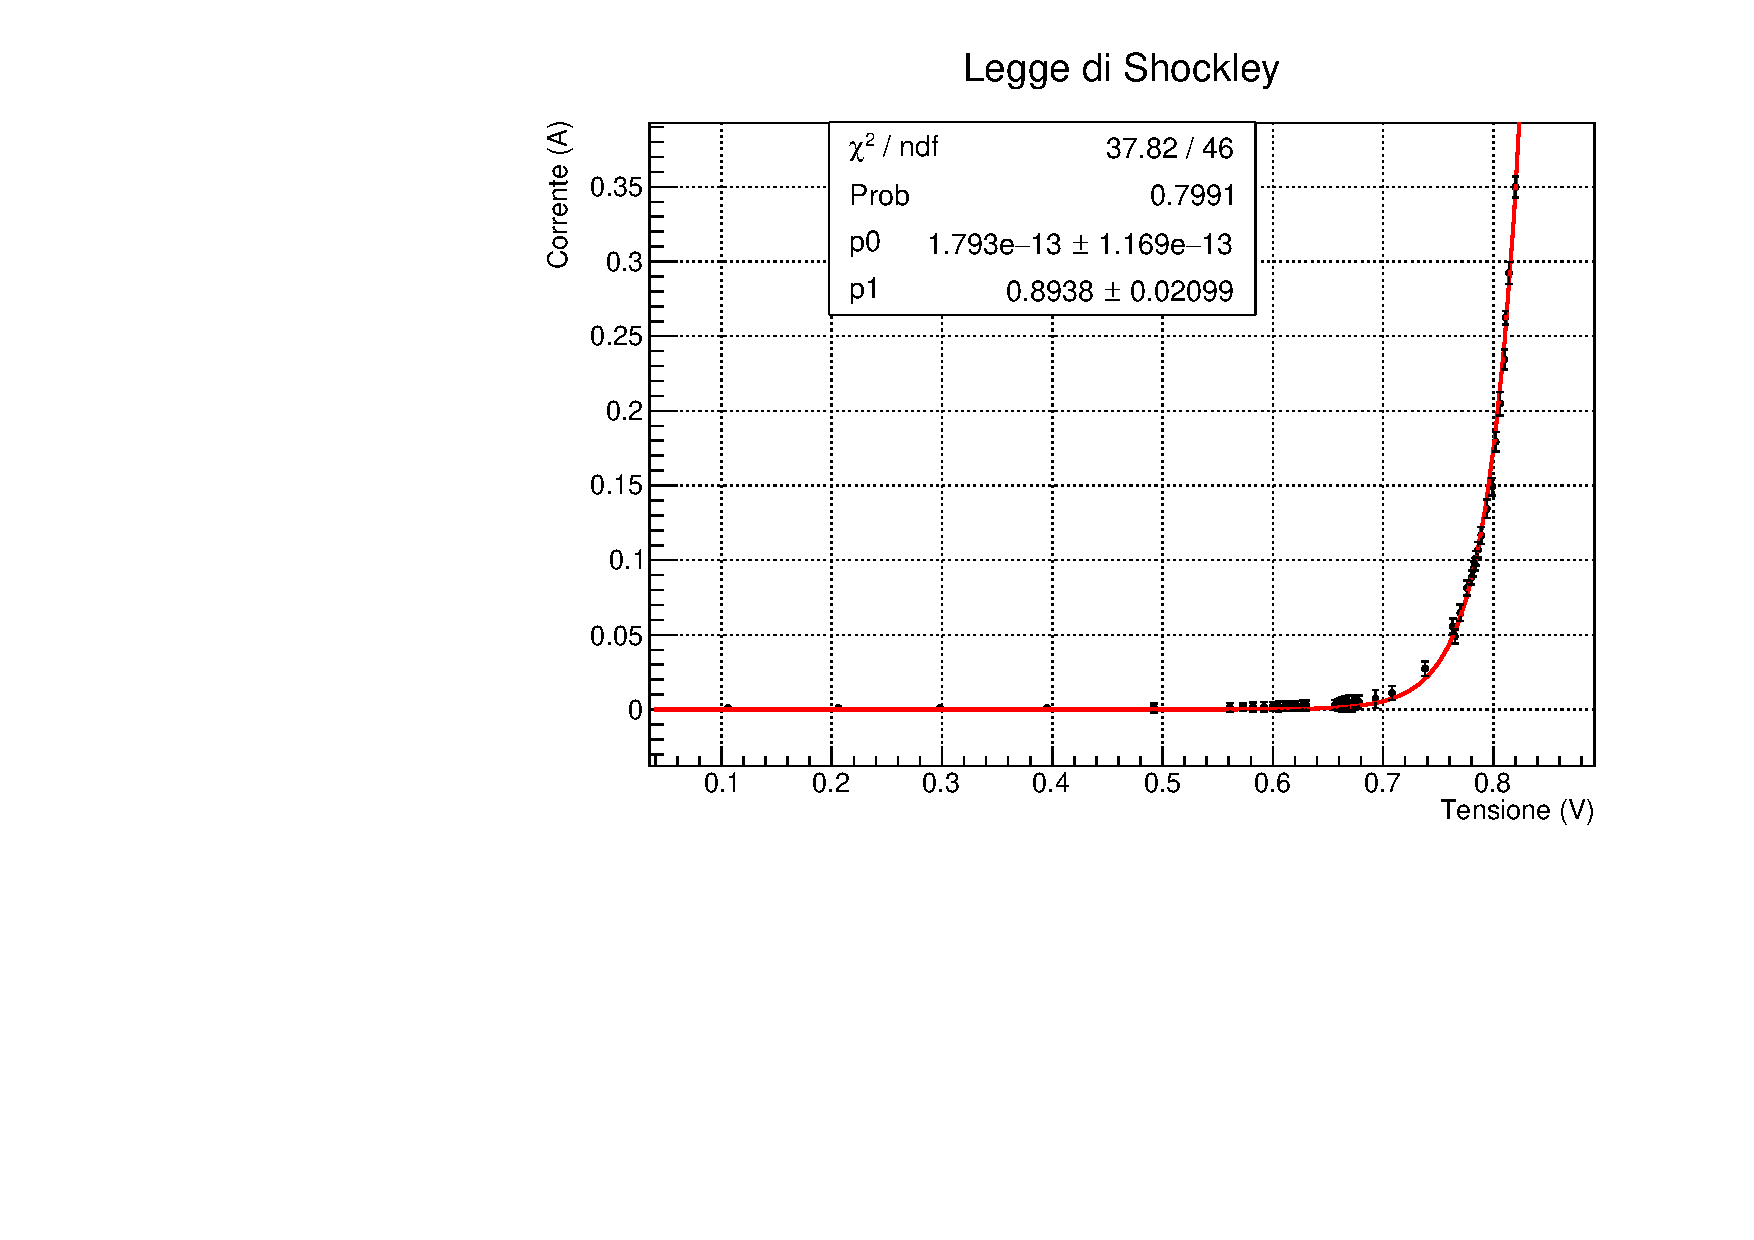
\includegraphics[scale=.5]{Immagini/diodo2.pdf}
    \caption{Fit con la legge di Shockley}
\end{figure}
In secondo luogo abbiamo individuato la $V_{soglia}$, fittando i dati con una retta, partendo dal range superiore delletensioni, fino a raggiungere un $\chi ^{2}$ ridotto di circa 1. Trovando l'intercetta di questaretta con l'asse \textit{x}, abbiamo ricavato $V_{soglia}$. Inoltre il parametro $p_0$ indica la corrente di saturazione che risulta essere dell'ordine del $10^{-13}$ come previsto dal modello teorico, mentre il parametro $p_1$ esprime il valore del rapporto $\frac{1}{g}$ dove $g$ è una costante che dipende dal materiale componente il diodo, pari circa a $1$ per diodi in germanio mentre circa $2$ per diodi in silicio. Da questo dato ricaviamo che $g\approx 1$ per cui l'ipotesi che il diodo sia composto da germanio risulta essere giustificata.
Di seguito è riportato il grafico con il fit della retta:

\begin{figure}[h!]
    \centering
    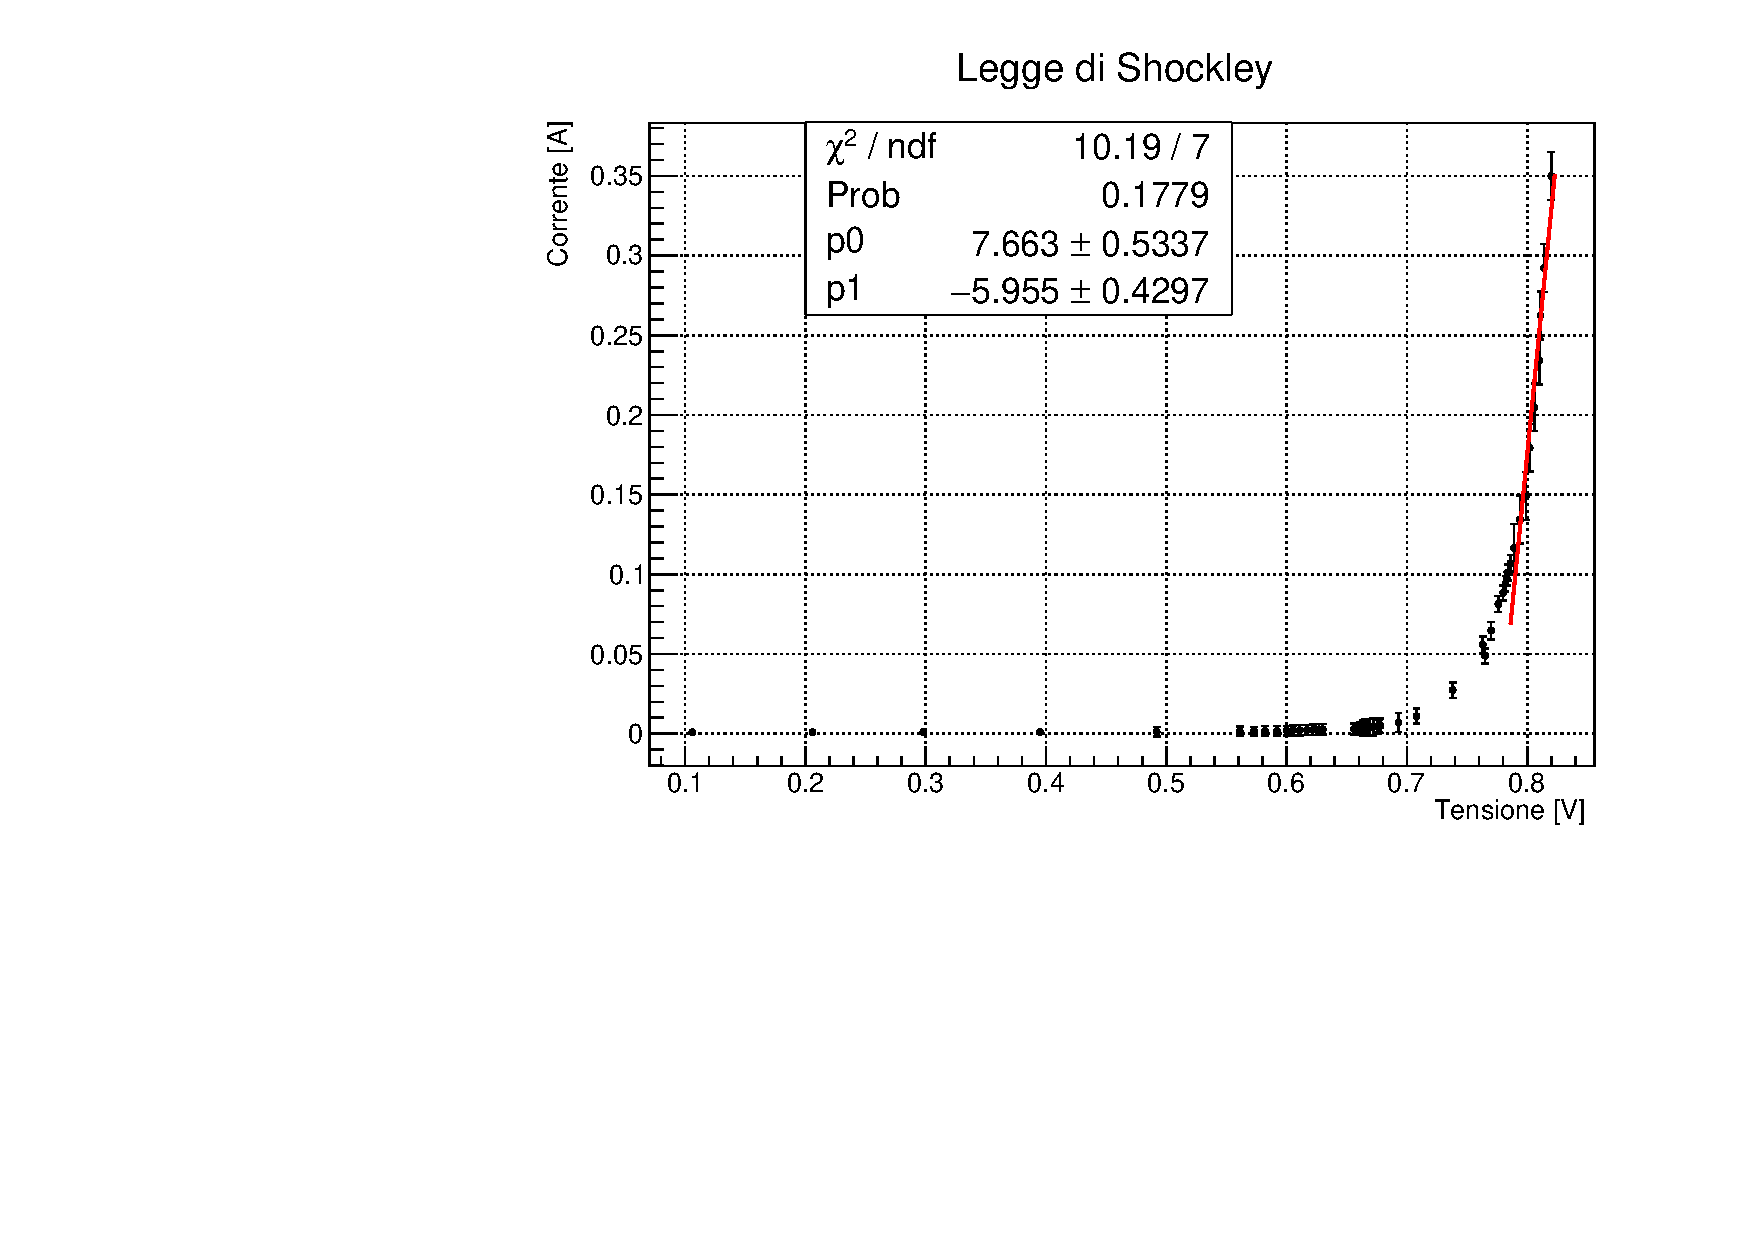
\includegraphics[scale=.5]{Immagini/diodo_soglia2.pdf}
    \caption{Fit con il diodo in conduzione da cui si ricava $V_{\text{soglia}}$ che corrisponde con il parametro $P_0$}
    \label{fig:my_label}
\end{figure}
\section{Conclusioni}
Lo scopo di questa esperienza è stato quello di studiare e verficare relazioni e leggi riguardanti resistenze e diodi. In primo luogo è stata condotta una verifica sulle due configurazioni, quella con il voltmetro e quella con l'amperometro, al fine di analizzare i loro comportamenti rispetto alle configurazioni ideali. Per l'amperometro i risultati ottenuti risultano congruenti con quelli aspettati, cosa che invece non accade con il voltmetro. Crediamo che la causa di ciò possa essere dovuta a due principali fattori. In primis riteniamo possibile che la resistenza scelta, la quale era necessario fosse confrontabile con quella del voltmetro, potrebbe non essere stata tale e che, quindi, l'errore sull'ordine di grandezza potrebbe essere stato causato da quello. Come seconda fonte di errore riconduciamo il fatto che, per identificare le resistenze, ci siamo serviti del tool online menzionato nell'introduzione, i cui valori potrebbero non corrispondere a quelli reali, inserendo quindi un possibile errore sistematico nei nostri risultati. A causa di tale incongruenza, in esperienze che fornivano la possibilità di scegliere la configurazione, abbiamo sempre preferito utilizzare quella con l'amperometro. Lo studio sulla relazione evidenziata da Ohm risulta corretta, nonostante il $\chi^2$ risulti molto bassa. La causa più probabile di questo fenomeno potrebbe essere ricercata in una sottostima degli errori, dovuta al nostro modo di identificare i valori delle resistenze. Nonostante questa possibile fonte di errore, lo studio sul partitore resistivo ha portato risultati congruenti rispetto al nostro studio teorico riguardo alle relazioni sulle resistenze. Infine, anche l'analisi sul diodo risulta congruente rispetto alla relazione ipotizzata, con un $\chi^2$ ridotto di circa 0.82. Riteniamo che l'esperimento potrebbe essere riprodotto con risultati più soddisfacenti se si procedesse a misurare le resistenze in maniera differente. 


\end{document}